\chapter{Control of mobile manipulator }
\label{c5_DI2}
In this chapter the control architecture of the teleoperated  mobile robot is presented. The user interface for teleoperation is discussed. The control algorithm  running on the mobile robot and the hardware used for the control of traction and steering is discussed. The protocol used  for communication between the robot and user interface also described in detail.
\section{Control Architecture and Hardware}


\begin{figure}
	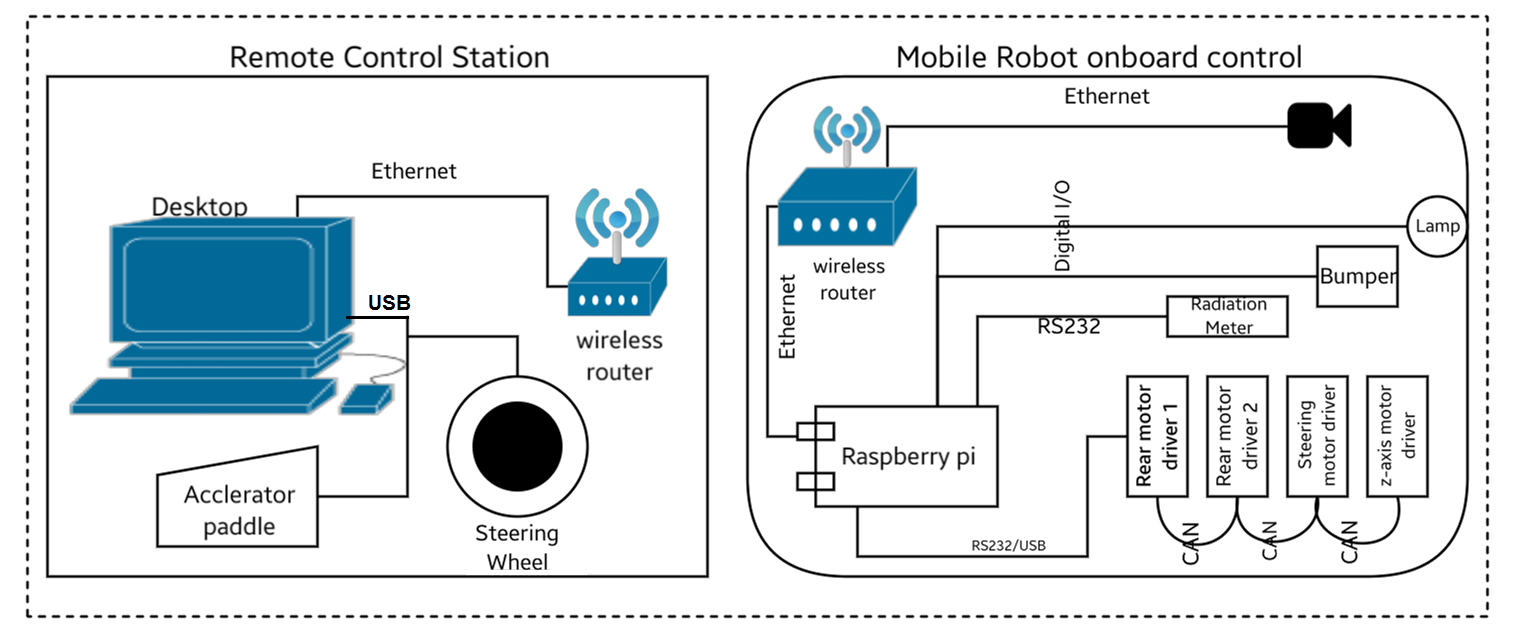
\includegraphics[width=\linewidth,keepaspectratio]{Chapter3/fig/controlblock}
	\captionof{figure}{Control Architecture Block Diagram }
	\label{fig:ControlBlockDiag} 
\end{figure} 
The mobile manipulator is planned to be teleoperated over a wireless network. The control block diagram and architecture are shown in Figure \ref{fig:ControlBlockDiag}. It has a remote control station which is the interface for the operator and a local controller on the mobile manipulator. They  communicate over dedicated wireless network. The remote station send data packet every 50 millisecond (20Hz) to the mobile manipulator. The commanded velocity, the steer angle, the z position of the platform and the state of the detector and headlamps constitutes the data packet sent by the remote station as shown in \ref{fig:sentBytes}. The on board control of the mobile robot replies with a data packet consisting of the $X$, $Y$ position and orientation $\theta$ of the robot, the current steer angle, angular velocities of each wheels, the z position of the top platform,  battery voltage  and current of each motor.


\subsection{Local Onboard Controller}
The  on-board computer which is Raspberry Pi running raspian (linux) os receives the command from the remote station and controls the robot hardware through customized c++ application.
The raspberry pi  is daisy chained to the four Maxon EPOS2 motor controllers/drivers. The communication between the onboard computer and the first Maxon controllers is over usb/RS232 interface using Maxon's proprietorial protocol~\cite{maxonrs232}. The first controller serves as CAN master for the rest of the controllers. The rear wheel motor drivers are configured in velocity servo loop. The steering and the z-axis motors drivers are configured in position control loop.  The camera mounted on the mobile robot  and Raspberry Pi  is connected over Ethernet via a wireless hub. the wiring digram of the robot is given figure \ref {fig:wiring}. Since the onboard camera is connected to the wireless net work directly, therefore it does not interfere with the command loop between the raspberri Pi and the PC. 

The mobile robot is teleoperated using position-speed command as in \cite{farkhatdinov2007hybrid} is used as the work space for the mobile robot is infinite compared to input device. In case of manipulators position-position control approach is used with scaling. In our case we user the mixed approach. The steering angle is controlled in position -position mode where as the mobile robots speed is controlled by foot paddle's position, i.e. position-velocity mode. This is given by the following equation 
\begin{equation}
	\begin{pmatrix}
	V\\\theta_S
	\end{pmatrix}=
	\begin{pmatrix}
	K_v & 0\\0 & K_s
	\end{pmatrix}
	\begin{pmatrix}
	\tilde{X_p}\\
	\tilde{\Theta_s}
	\end{pmatrix}
\end{equation}
where $\tilde{X_p}$ is the displacement of  paddle, $\tilde{\theta_s}$ is the twist in steering wheel, $K_v$ and $K_s$ are the proportionality constants, $V$ is the velocity of point $O_3$ and $\theta_s$ is the displacement of the steer motor. These proportionality constants are derived as below bases on extreme limits. 

\begin{table}[!htbp]
	\caption{Proportionality constant table}
	\centering
	\begin{tabular}{l l l l l}
		\hline
		Robot  & range & Joy-Stick& range & parameter \\
		parameters& & Parameter & & Value\\
		\hline
		$\theta_s$ & -60 to +60 & $\tilde{\Theta_s}$ & $-90^o$ to $90^o$ & $K_s=2/3$\\
		$V$ & 0 to +60 mm/sec & $\tilde{X_p}$ & 0 to 30mm & $K_v=2$\\
		\hline
	\end{tabular}	
\end{table}

\begin{figure}
	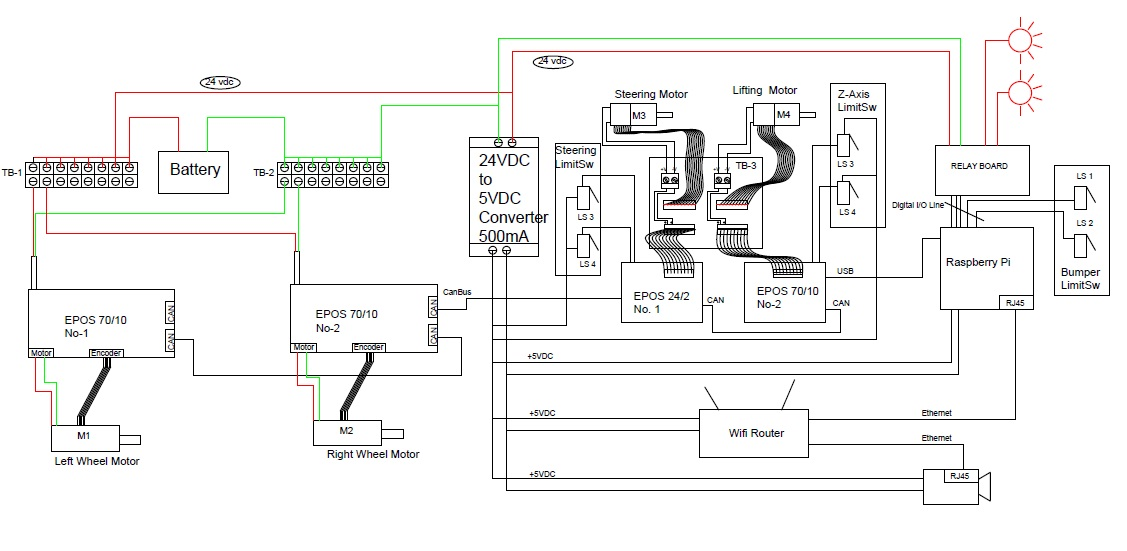
\includegraphics[width=\linewidth,keepaspectratio]{Chapter5/fig/RobotSideWiring}
	\captionof{figure}{Wiring  Diagram of Robot }
	\label{fig:wiring} 
\end{figure} 
\subsection{Details of Motor Controller}
Three EPOS2 controller from Maxon Motors is used to control the mobile robots rear wheel velocity and the steering gear position. Each controller can control one motor. The over architecture of the controller  as given in \cite{maxonAutoTune}, \cite{maxonAppNotesPosition} and is shown here in  figure \ref{fig:EPOS4}. The controller can be configured in either current, position or velocity control mode. The inner most current loop controls the torque of the motor.
 The current feedback loop shown in figure \ref{fig:curloop} is a PI loop running at 25KHz and the transfer function of the PI block is given in equation \ref{eqn:curLoop}. 
 \begin{equation}
 	C(s)=K_p + \frac{K_I}{s}
 	\label{eqn:curLoop}
 \end{equation}
 where $K_p$ and $ K_I$ are the proportional and Integral gains.
   \begin{figure}
 	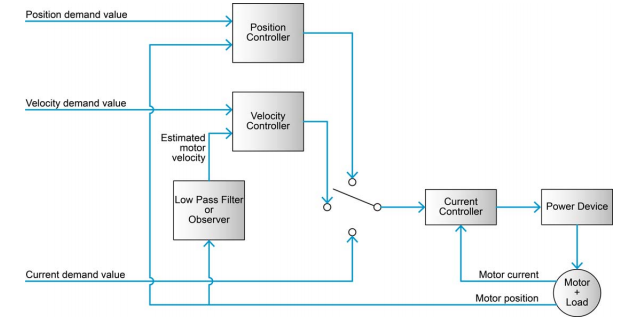
\includegraphics[width=\linewidth,keepaspectratio]{Chapter5/fig/overallcontorl}
 	\captionof{figure}{EPOS4 Controller Block Digram }
 	\label{fig:EPOS4} 
 \end{figure}
 \begin{figure}
 	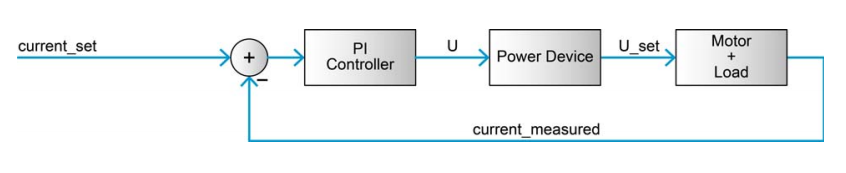
\includegraphics[width=\linewidth,keepaspectratio]{Chapter5/fig/currentLoop}
 	\captionof{figure}{Current control bolck digram }
 	\label{fig:curloop} 
 \end{figure}
 
 
  The rear motor controllers are configured to  in velocity mode.  The block digram  of the velocity loop is given in figure \ref{fig:velloop}. The velocity controller is a PI controller with  velocity and acceleration feed-forward. The transfer function $V(s)$of velocity loop PI block is given by
  \begin{eqnarray}
  V(s)=K_{p\omega}+\frac{K_{I\omega}}{s}
  \end{eqnarray}  where $K_{p\omega}$ and  $K_{I\omega}$ are velocity proportional and integral gain respectively.
   The sampling rate of the  velocity loop is 2.5 KHz. The feedforward accleration and feedforward velocity is used to compensate for the known inertial load and  viscous frictional load  \cite{maxonAppNotesPosition}.  The lowpass filter used in \ref{fig:EPOS4} is used  because velocity is estimated from differentiating  the position, the filter eliminates noise due to differentiation. The transfer function $H(s)$ of  lowpass filter is given below
  \begin{equation}
  H(s)=\frac{1}{1+\frac{K_{p\omega}}{48K_{I\omega}}}
  \end{equation} 
  The gain values used for each rear motor in  the velocity control mode is listed in table \ref{tb:Left} and \ref{tb:Right}. No acceleration or velocity feedforward  was used. These parameters were determined by auto tuning.  
  \begin{table}[!htbp]
  	\caption{ Rear Right Motor Controller  parameters }
  	\label{tb:Right}
  	\centering
  	\begin{tabular}{l l l}
  		\hline
  		\emph{Gain Parameter}  & \emph{ Value} & \emph{Unit} \\
  		\hline
  		$K_p$  & 300 &  $\frac{mV}{A}$ \\ 
  		$K_I $ & 100 & $\frac{mV}{A.mS}$ \\
  		$K_{P\omega}$& 1000 & $ \frac{mA.sec}{rad}$\\
  		$K_{I\omega}$&100&$\frac{mA}{rad}$\\
  		\hline
  	\end{tabular}
  \end{table}
  \begin{table}[!htbp]
  	\caption{ Rear Right Motor Controller  parameters }
  	\label{tb:Left}
  	\centering
  	\begin{tabular}{l l l}
  		\hline
  		\emph{Gain Parameter}  & \emph{ Value} & \emph{Unit} \\
  		\hline
  		$K_p$  & 230 &  $\frac{mV}{A}$ \\ 
  		$K_I $ & 53 & $\frac{mV}{A.mS}$ \\
  		$K_{P\omega}$& 5182 & $ \frac{mA.sec}{rad}$\\
  		$K_{I\omega}$&425&$\frac{mA}{rad}$\\
  		\hline
  	\end{tabular}
  \end{table}

\begin{figure}
	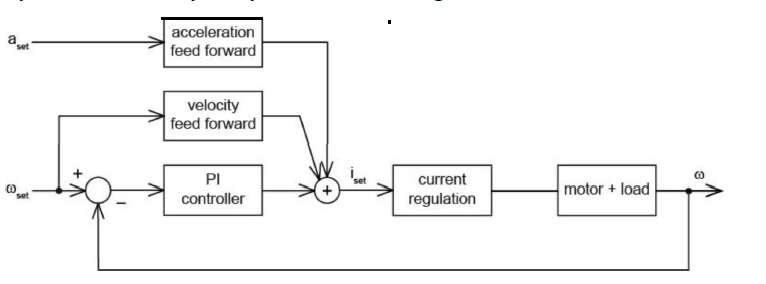
\includegraphics[width=\linewidth,keepaspectratio]{Chapter5/fig/velLoop}
	\captionof{figure}{Velocity control bolck digram }
	\label{fig:velloop} 
\end{figure}
\begin{figure}
	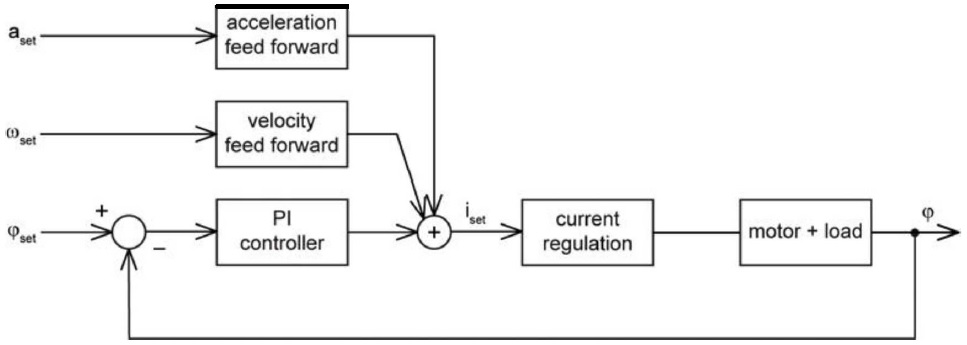
\includegraphics[width=\linewidth,keepaspectratio]{Chapter5/fig/posLoop}
	\captionof{figure}{Position control bolck digram }
	\label{fig:posloop} 
\end{figure}


The steering motor is in position control mode. The block digram is shown in figure \ref{fig:posloop}. It is a PID controller with transfer function given as 
\begin{equation}
P(s)=K_{PP}+K_{IP}s+\frac{K_{DP}s}{1+\frac{K_{DP}}{10 K_{PP}}s}
\end{equation}
where $K_{PP}$, $K_{IP}$ and $K_{DP}$ are position proportional, integral and derivative gains. The velocity $F_{\omega P}$ and acceleration $F_{\alpha P}$ are also used in position control loop to take care of viscious friction and known inertial load. The gains for controller was decided using auto tuning software provided by Maxon Motors. The value are reported in table \ref{tb:steer}.

\begin{table}[!htbp]
	\caption{ Rear Steer Motor Controller  parameters }
	\label{tb:steer}
	\centering
	\begin{tabular}{l l l}
		\hline
		\emph{Gain Parameter}  & \emph{ Value} & \emph{Unit} \\
		\hline
		$K_p$  & 537 &  $\frac{mV}{A}$ \\ 
		$K_I $ & 307 & $\frac{mV}{A.mS}$ \\
		$K_{PP}$& 128 & $ \frac{mA.sec}{rad}$\\
		$K_{IP}$&663&$\frac{mA}{rad}$\\
		$K_{ID}$&200&$\frac{mA}{rad}$\\
		$F_{\omega P}$& 0& $ \frac{mA.sec}{rad}$\\
		$F_{\alpha P}$& 54& $ \frac{mA.sec^2}{rad}$\\
		\hline
	\end{tabular}
\end{table}
\subsection{The control Algorithm}
Thsi section discusses the in detail the algorithem running of the on-board controller.  Command received by the controller is parsed to extract the velocity  and the steer angle  information and suitably scaled to get command velocity  $V$, in mm/sec and steering  angle $\theta_s$ in radians.  It may be noted that the velocity $v$ corresponds to the velocity of point $O_r$ the reference point of the mobile robot.  Next based the set point for each motor is calculated  and sent to individual drives. The algorithm is listed below and the block digram for the same in figure \ref{fig:ControlBlock}
\begin{figure}
	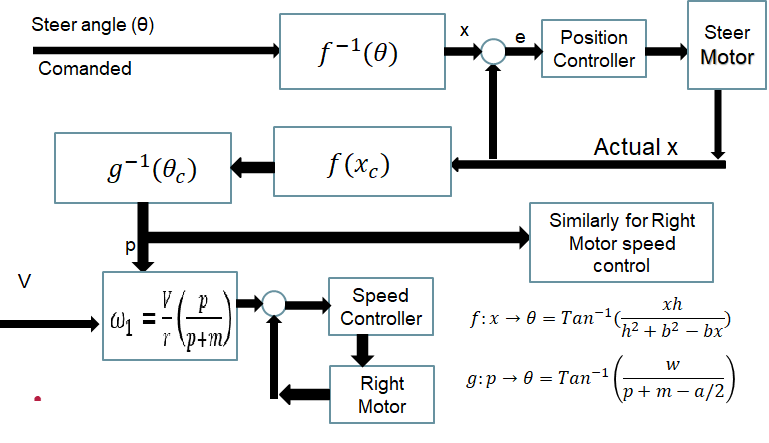
\includegraphics[width=\linewidth,keepaspectratio]{Chapter5/fig/BlkDigLocal}
	\captionof{figure}{provide suitable title }
	\label{fig:ControlBlock} 
\end{figure}

\begin{enumerate}
	\item Calculate the rear wheel velocities setpoints $\omega_{RS}$ and $\omega_{LS}$ based on the $V$ and $\theta_s$
	\item Read the current rear wheel velocities $\omega_{LC}$ and $\omega_{RC}$
	\item Calculate the setpoint for steering motor $\theta_{ss} $
	\item sent setpoints $\omega_{RS}$,$\omega_{LS}$ and $\theta_{ss} $ to each motor 
\end{enumerate}

It may be noted that the steer angle command received from the control station is not directly sent to the steer motor as set point after suitable scaling. The steer set point is based on the current rear wheel velocities. This important as the response time of the  motors are different. The above methodology helps  minimize deviation  from the Ackerman  steering condition even during transit condition, particularly in case of large change in commanded $v$ and $\theta_s$. 
Each block in the figure \ref{fig:ControlBlock} is discussed next. 

 It may be noted that the $\theta_s$ always refers to the steer angle of the inner front wheel $\phi_i$ as shown in figure \ref{fig:KenVrc}, i.e.
 \begin{equation}
	 \theta_s =\phi_i
 \end{equation}
 The set point of the steering motor at the output of  gear box $\theta_{SM}$ is given by equations \ref{eqn:sterineq1} and \ref{eqn:sterineq2}  based on the geometry of Davis steering gear \cite{TOMBook}.
\begin{equation*}
 \tan\phi_i=\frac{xh}{h^2+b^2-bx}
\end{equation*}
or
\begin{eqnarray}
f:\phi_i\rightarrow x, \quad x=\frac{\tan\phi_i (h^2+b^2)}{h+b \tan\phi_i }
\label{eqn:sterineq1}
\end{eqnarray}
where $x$ is the displacemet of the rack and $h$ and $b$ are link lengths. The rack is connected to the steering motor by pinion of pcd ($D_p$) 30mm as shown in the figure \ref{steering_gear_train}. Therefore the set point for the steering motor is given below as
\begin{eqnarray}
\theta_{SM}= x \frac{360}{\pi D_p}
\label{eqn:sterineq2}
\end{eqnarray}
 
Next we present  the equation relating current steer angle $\phi_{ic}$ which  and rear wheel  set point velocities. From the geometry of figure \ref{fig:kinVec} we get
\begin{align}
\nonumber \tan\phi_i &=\frac{\bar{BD}}{\bar{OB}}=\frac{w}{p+m-a/2}\\ 
p &= \frac{w}{\tan\theta_o}-m + \frac{a}{2}
\end{align}
%similarly for the inner wheel we get  
%\begin{equation}
%p = \frac{w}{\tan\theta_i}-m - \frac{a}{2}
%\end{equation}
now from the rear wheel velocity digram we get
\begin{align}
\nonumber \frac{\omega_i r}{p}&=\frac{\omega_o r}{p+2m}=\frac{v}{p+m}\\
\omega_i &=\frac{vp}{p+m}\\
&=\frac{v( \frac{w}{\tan\theta_o}-m + \frac{a}{2})}{ \frac{w}{\tan\theta_o}-m + \frac{a}{2}+m}
\end{align}
  
\begin{figure}
	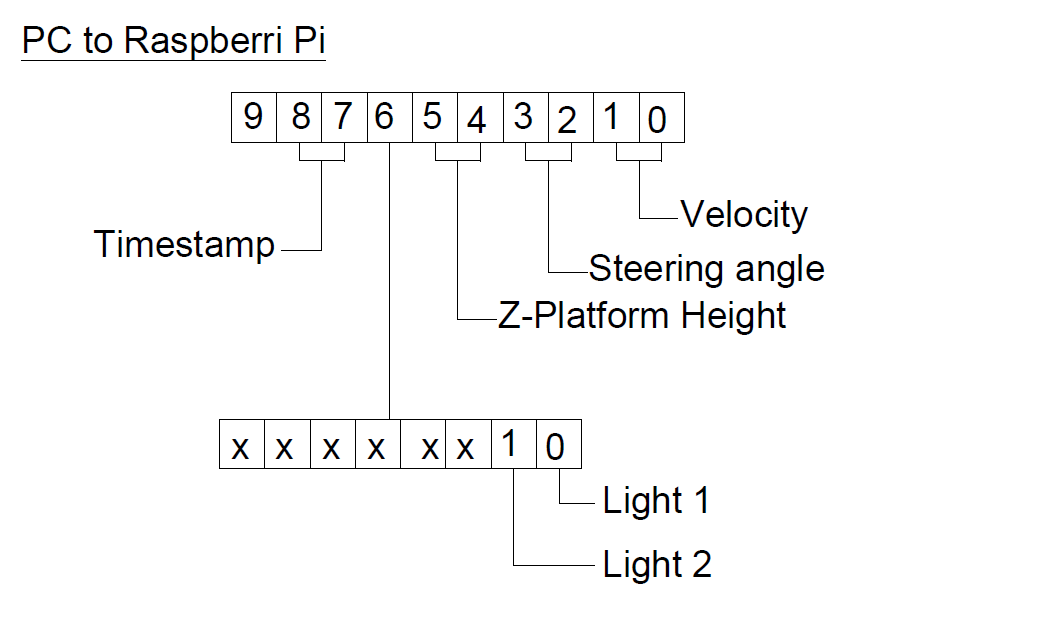
\includegraphics[width=\linewidth,keepaspectratio]{Chapter5/fig/bitconfig}
	\captionof{figure}{Data sent from PC to Onboard controller }
	\label{fig:sentBytes} 
\end{figure}
 
\begin{itemize}
\item steering kinematic equation
\item Sequence of program flow
\item data structure of command  and  frequency
\item calibration of steer data and wheel velocity
\end{itemize}
\subsubsection{Control of Z platform}
Decentralized control technique treats the manipulator and the platform as two different system. The inter-coupling forces are treated as external forces on the system. The dynamics equation of the mobile manipulator can thus be split as follows [3]
\subsubsection{Odometry }
The dead reconning odometery can be performed based on the differential wheel model ot the bicycle model.
\subsection{The Remote Control Station}   
The local station consists of a desktop computer running Windows XP. A Steering wheel and two foot switches are connected to the desktop. The steering wheel is used for turning  mobile robot. One of the two foot switch acts as an accelerator to set the mean velocity the other  is used to brake the vehicle.

The screen of the desktop displays the video streaming  from the mobile robot on board camera. A graphical user  interface (GUI) also displays the robot's parameters such as current steer angle, velocity of each rear wheel and the position of the z-axis. Buttons on the GUI operates the z-axis, head lamps, etc.

\begin{figure}
	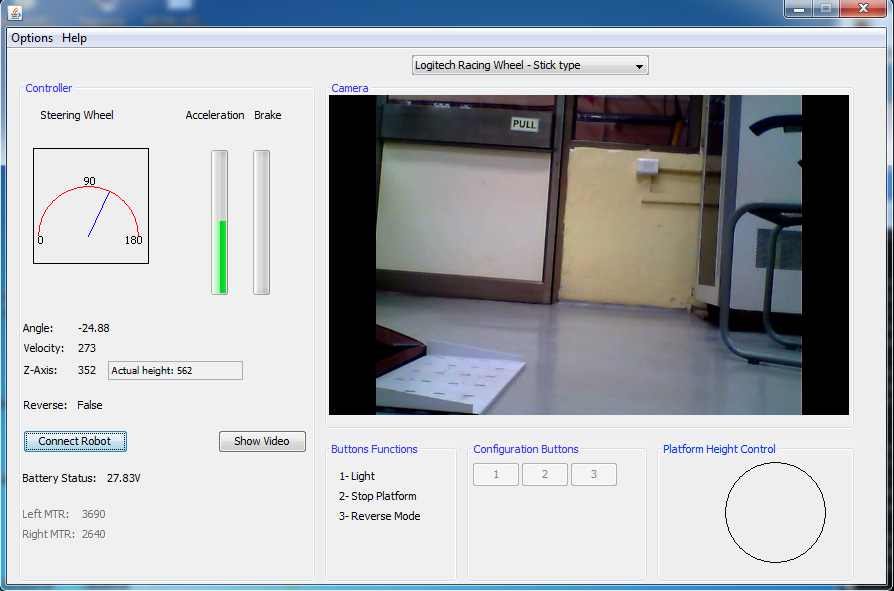
\includegraphics[width=\linewidth,keepaspectratio]{Chapter5/fig/gui}
	\captionof{figure}{User Interface for teleoperation }
	\label{fig:Gui} 
\end{figure}

%\section{Admissible path}
%\section{Trajectory Tacking}


\section{Summary}
In this chapter, 